\documentclass[twocolumn,10pt,a4paper]{article}
\usepackage[T1]{fontenc}
\usepackage[utf8]{inputenc}
% \usepackage[ngerman]{babel}% war auskommentiert fuer den Satz
\usepackage{times}
\usepackage{verbatim}
\usepackage{moreverb}
\usepackage{alltt}
%  \usepackage{nofloat,lstfloat}
\usepackage{float}
\usepackage{url}
\usepackage{graphicx}
\def\UrlFont{\tt\small}
\title{Interfacing with RHQ}
\author{Heiko W.\ Rupp}
\begin{document}
\sloppy
\maketitle



\begin{abstract}
RHQ\footnote{\url{http://rhq-project.org/}} is an open source software suite that manages and monitors any resource able to communicate with the suite.

In RHQ terms, a \emph{resource} 
is everything that can be monitored or managed. Examples are java processes, a datasource within an application server or disks and cpu of a machine, but could also be thermometer chips or light sensors.

Functionality of RHQ includes:
\begin{itemize}
\item Auto-detection of managed resources
\item Monitoring of resource metrics, logfiles, or other event sources. This also includes graphing of metrical values. Metrical values are stored for up to a year.
\item Configuring the managed resources
\item Running operations against resources
\item Deploying software ("Bundles") onto managed machines
\item Alerting on metrical values, operation outcome, and many more conditions
\item Detection of filesystem content changes ("Drift")
\item Grouping of resources in order to issue operations on the whole group
\end{itemize}

RHQ has been designed with extensibility in mind. 
In order to support managed resources that are not delivered out of the box 
(e.g.\ other kinds of servers or network equipment etc.), 
the user can write plugins that interface with those resources, and add them to RHQ.

This paper gives a short overview of RHQ and its architecture, and then
describes the ways to interface with RHQ.
\end{abstract}

\section{Overview}
RHQ consists of a central server (or cluster of servers) and so called
\emph{agents} on managed machines (\emph{platforms} in RHQ terminology) and thus
follows a hub and spoke approach. Connected to the server is the central
database that stores the inventory -- the list of managed resources, gathered
metrics, schedules for operations to be executed, and much more.

\noindent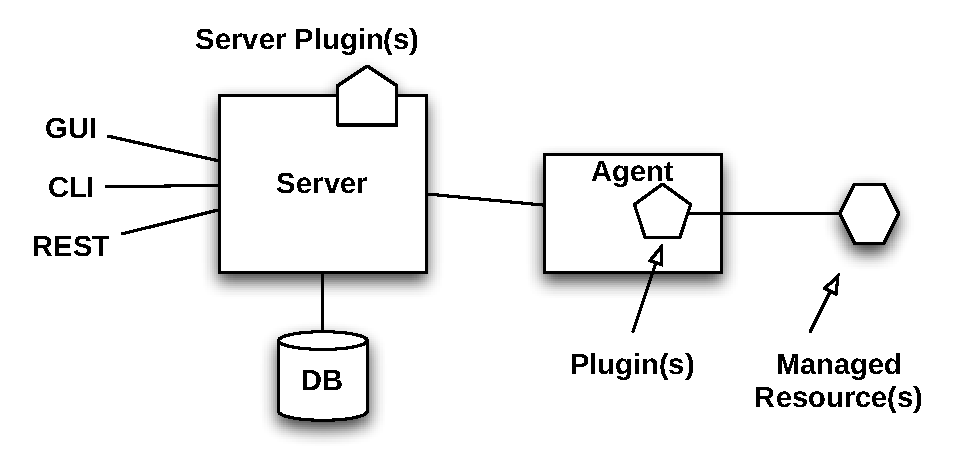
\includegraphics[width=\columnwidth]{graph/arch.pdf}

All user interaction with RHQ also happens on the server, be it via the graphical
user interface, the command line interface or via REST. 

Agents connect to the server and themselves host the \emph{agent plugins} (often
just called "plugins") which do the actual work of interfacing with the managed
resources; the server never talks to managed resources directly.

A second kind of plugin, the \emph{server plugin}, runs in the server; most
prominent server plugins are alert notification senders that are invoked when an
alert is fired.

\section{Graphical user interface}

The main interface for RHQ is a graphical user interface that is for the most part
written with the Google Web Toolkit (GWT). There are still some older parts that use other
technologies. The GUI can be reached at \url{http://localhost:7080/}; default
username and password after installation are 'rhqadmin' and 'rhqadmin'. The UI
has been partially translated into several languages like Japanese, Chinese, Portuguese or German. After logging in, you are presented with a dashboard, that gives an
overview of the system state.

\section{Command line interface}

The command line interface is another way to communicate with RHQ. The user can run the CLI interactively to explore the system or can pass pre-created scripts to it to be executed.

The programming language inside the CLI is JavaScript\footnote{There is 
a proof of concept that uses other programming languages like Ruby for this 
purpose, so in theory one would not be restricted to JavaScript.}, where 
several of the server methods have been made available as built-in functions. 
This allows users to write powerful scripts with loops, conditions, and other logic.

\section{Agent plugins}

Agent plugins implement the logic to communicate with managed resources.
The plugin iteself consists of some Java code and metadata in XML, the 
so-called \emph{plugin descriptor}, which tells the agent\footnote{More precisely, 
the plugin-container which runs inside the agent and which actually 
hosts the plugins is given the metadata.} what functionality is 
available. A plugin does not need to implement all \emph{facets} of 
management and can pick several aspects. The plugin descriptor 
wires those together. It also tells the server what functionality 
a plugin provides, so that the server can dynamically render the 
UI from this metadata. This also implies that the server itself 
has no built-in knowledge about any managed resource.

\subsection{Parts of an agent plugin}

An agent plugin consists of three parts:
\begin{itemize}
\item Discovery mechanism: this reaches out to managed resources, finds them and reports them back to the system.
\item Component mechanism: this implements the various facets of functionality.
\item Plugin descriptor: this defines the functionality and wires the components together
\end{itemize}

If you want to learn more about plugin development, you can refer to the documents in the "Further reading" section.

\section{Server plugins}

Server plugins are a relatively general concept to extend the server functionality. The most prominent use case in RHQ are the alert notification sender plugins. 

When RHQ fires an alert, it will call the configured alert senders to do the actual notification. This can be via email or SNMP\footnote{Simple Network Management Protocol} trap, as those are senders that come with RHQ out of the box.\footnote{Other alert protocols can be configured and installed.}

As the alert notification senders are server side plugins you can write your own integrations to other monitoring systems or to SMS gateways, for example. In many enterprises, all alerts need to be logged in a central trouble-ticket system. The plugin can create this interface and do a REST-PUT request into the trouble ticket system.

Other kinds of server plugins include content sources or report generation: server plugins can be triggered at regular intervals so it is also possible to generate hourly reports about deployed systems and send them via email. 

Server side plugins could also read external files and compute memberships of resource groups from the data in this file.

\section{REST Interface}

The REST interface provides a way to retrieve values and store 
new values in the server in a language-agnostic way.
This allows users to \emph{manage the enterprise with curl}, if so desired. 
One of the more
popular use cases involving the REST API is the creation of custom dashboards where many metrical
graphs are displayed on a huge screen; this can be achieved with the help
of some JavaScript code or the D3.js\footnote{\url{http://mbostock.github.com/d3/}} library, for example.

\noindent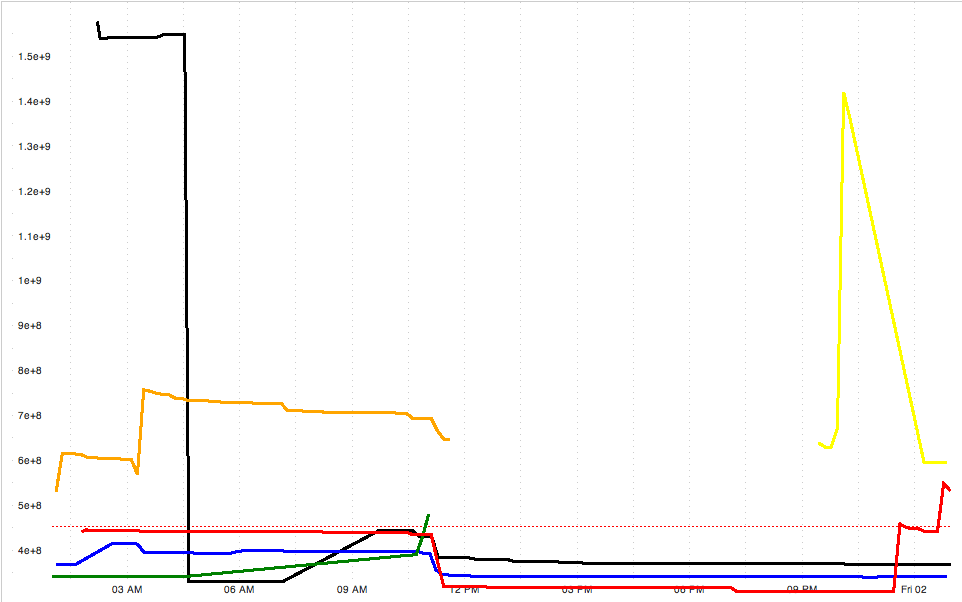
\includegraphics[width=\columnwidth]{graph/multigraph.png}

While currently not complete, it will contain a good part of the functionality
that is needed for daily business; just recently export of the reports (suspect metrics, recent alerts etc.) has been added. 

The REST API is clearly intended to be read-write. In fact it is possible to supply metric or baseline data values from external sources. 

The next diagram shows a metric graph with two baselines (lower and upper). By default those are computed in the RHQ server to be the min and max values for the metrics in the last \emph{n} days. Near the end the metric goes above the upper baseline and thus generates an out-of-band (OOB) event.

\noindent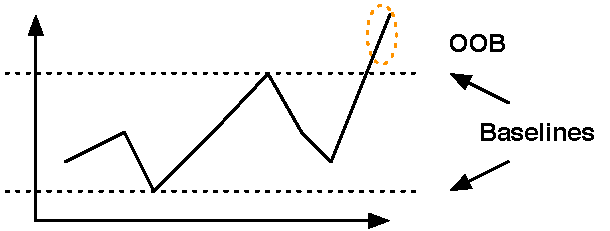
\includegraphics[width=\columnwidth]{graph/baseline_graph.pdf}

It is also possible to turn the automatic baseline calculation off and have an external system supply those values via the REST API:

\noindent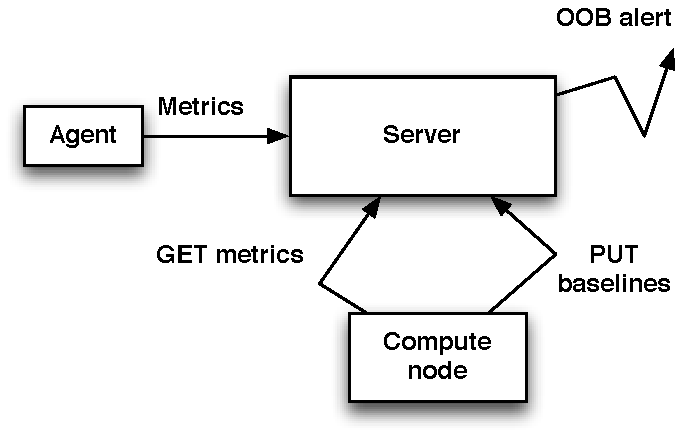
\includegraphics[width=\columnwidth]{graph/ext_baseline.pdf}

In this example, we see the agent still delivering metrics as usual. The compute node calls into the server and requests the raw metrics from the most recent day and then computes baselines for those values, which are then fed into the RHQ server, which will then use those baselines for alert generation. Interesting candidates to compute the baseline are for example 1\% and 99\% quantiles of the metric values or a computation\footnote{The Holt-Winters method is one exponential smoothing computation that accounts for expected variations in data.} that is able to take seasonal variations (weekday vs.\ weekend) into account.

\section{Further reading}

There is a lot of documentation available for RHQ. The main source of information is the Wiki at \url{http://rhq-project.org/}, which also links to most of the following resources:

\begin{itemize}
\item Video "Overview of RHQ 3" \url{http://vimeo.com/16424369}
\item Video "How to write a plugin" \url{http://vimeo.com/16171314}
\item Whitepaper "How to write a plugin": this gives a step by step introduction into plugin writing. While it is a bit old most parts still apply to current versions of RHQ
\item RHQ user documentation \url{http://rhq-project.org/display/JOPR2/Home}
\end{itemize}

In addition a big part of the documentation for JBoss Operations Network (JBoss ON) applies to RHQ as well. This documentation can be found at \url{http://docs.redhat.com/docs/en-US/JBoss_Operations_Network/3.0/}

\end{document}
